% ============================================================
%  SCHOLA DOMESTICA — Magister Mathematica
%  Level 1 | Week 9 | Day 2
%  Topic: Addition Facts — Sums to 6 (+2 and +3)
% ============================================================
\documentclass[12pt, letterpaper]{article}

\usepackage[top=1in, bottom=1in, left=1in, right=1in]{geometry}
\usepackage[T1]{fontenc}
\usepackage[utf8]{inputenc}
\usepackage{lmodern}
\usepackage{microtype}
\usepackage{amsmath}
\usepackage{amssymb}
\usepackage{graphicx}
\usepackage{xcolor}
\usepackage{tikz}
\usepackage{array}
\usepackage{booktabs}
\usepackage{enumitem}
\usepackage{multicol}
\usepackage{mdframed}
\usepackage{fancyhdr}
\usepackage{calc}

\definecolor{scholared}{RGB}{160,30,30}
\definecolor{scholagold}{RGB}{180,140,40}
\definecolor{scholacream}{RGB}{253,248,235}
\definecolor{scholagreen}{RGB}{50,110,60}
\definecolor{scholablue}{RGB}{40,80,140}

\pagestyle{fancy}
\fancyhf{}
\renewcommand{\headrulewidth}{0.6pt}
\fancyhead[L]{\small\textcolor{scholared}{\textbf{Schola Domestica — Magister Mathematica}}}
\fancyhead[R]{\small\textcolor{scholared}{Level 1 · Week 9 · Day 2}}
\fancyfoot[C]{\small\textcolor{gray}{— \thepage\ —}}

\newcommand{\answerline}{\underline{\hspace{2.5cm}}}
\newcommand{\biganswerline}{\underline{\hspace{4cm}}}
\newcommand{\numbox}{\tikz{\draw[scholablue,thick](0,0)rectangle(1.2cm,0.85cm);}}

\newmdenv[
  backgroundcolor=scholacream,
  linecolor=scholared,
  linewidth=1.5pt,
  roundcorner=6pt,
  innertopmargin=8pt,
  innerbottommargin=8pt,
  innerleftmargin=10pt,
  innerrightmargin=10pt
]{lessonbox}

\newmdenv[
  backgroundcolor={rgb,255:red,235;green,245;blue,235},
  linecolor=scholagreen,
  linewidth=1.2pt,
  roundcorner=4pt,
  innertopmargin=6pt,
  innerbottommargin=6pt,
  innerleftmargin=8pt,
  innerrightmargin=8pt
]{enrichbox}

\begin{document}

\begin{center}
  {\LARGE\textbf{\textcolor{scholared}{Addition Facts:}}}\\[4pt]
  {\Large\textcolor{scholagold}{\textit{Adding Two and Adding Three}}}\\[6pt]
  {\small Name: \biganswerline \hspace{1cm} Date: \answerline}
\end{center}

\vspace{4pt}
\noindent\textcolor{scholared}{\rule{\linewidth}{1pt}}
\vspace{4pt}

% IMAGE PROMPT (Beatrix Potter watercolour style):
% Two small rabbits each carry a basket. One basket holds two strawberries, the other holds three.
% They tip their baskets together on a grassy bank. Delicate watercolour, pale green and pink tones,
% white paper background, no text.

\begin{lessonbox}
\textbf{Strategies for $+2$ and $+3$:}\\[4pt]
\begin{itemize}[leftmargin=1.5em, itemsep=3pt]
  \item \textbf{$+2$}: count up \emph{two} steps from the first number.\\
        \hspace{1em} $3 + 2$: start at 3 … \textit{four} … \textit{five} \; $= 5$
  \item \textbf{$+3$}: count up \emph{three} steps.\\
        \hspace{1em} $1 + 3$: start at 1 … \textit{two} … \textit{three} … \textit{four} \; $= 4$
\end{itemize}
\medskip
\noindent\textit{You may use your fingers to count up!}
\end{lessonbox}

\bigskip

% ===== PART I: +2 WITH DOTS =====
\noindent\textcolor{scholared}{\large\textbf{Part I — Adding Two}} \hfill \textit{(Problems 1–6)}

\medskip
\noindent\textit{The blue dots are the first number. The gold dots are $+2$. Count all dots. Write the sum.}

\bigskip

\noindent
\begin{tabular}{@{}p{7.2cm} p{7.2cm}@{}}

% Problem 1: 1+2=3
\textbf{1.}\quad

\begin{tikzpicture}[baseline=-0.5ex]
  \filldraw[scholablue] (0.42,0) circle (0.14cm);
  \filldraw[scholagold] (0.97,0) circle (0.14cm);
  \filldraw[scholagold] (1.52,0) circle (0.14cm);
\end{tikzpicture}
\quad $1 + 2 =$ \numbox
&
% Problem 2: 2+2=4
\textbf{2.}\quad

\begin{tikzpicture}[baseline=-0.5ex]
  \foreach \i in {1,2} { \filldraw[scholablue] (\i*0.42,0) circle (0.14cm); }
  \foreach \i in {3,4} { \filldraw[scholagold] (\i*0.42,0) circle (0.14cm); }
\end{tikzpicture}
\quad $2 + 2 =$ \numbox \\[18pt]

% Problem 3: 3+2=5
\textbf{3.}\quad

\begin{tikzpicture}[baseline=-0.5ex]
  \foreach \i in {1,2,3} { \filldraw[scholablue] (\i*0.42,0) circle (0.14cm); }
  \foreach \i in {4,5} { \filldraw[scholagold] (\i*0.42,0) circle (0.14cm); }
\end{tikzpicture}
\quad $3 + 2 =$ \numbox
&
% Problem 4: 4+2=6
\textbf{4.}\quad

\begin{tikzpicture}[baseline=-0.5ex]
  \foreach \i in {1,...,4} { \filldraw[scholablue] (\i*0.42,0) circle (0.14cm); }
  \foreach \i in {5,6} { \filldraw[scholagold] (\i*0.42,0) circle (0.14cm); }
\end{tikzpicture}
\quad $4 + 2 =$ \numbox \\[18pt]

% Problem 5: 0+2=2
\textbf{5.}\quad $0 + 2 =$ \numbox
&
% Problem 6: 2+0=2 (review +0)
\textbf{6.}\quad $2 + 0 =$ \numbox \quad \textit{(review)}

\end{tabular}

\bigskip\bigskip

% ===== PART II: +3 WITH NUMBER LINE =====
\noindent\textcolor{scholared}{\large\textbf{Part II — Adding Three}} \hfill \textit{(Problems 7–12)}

\medskip
\noindent\textit{Hop forward 3 spaces on the number line. Write the sum.}

\bigskip

% Number line 0–6
\noindent
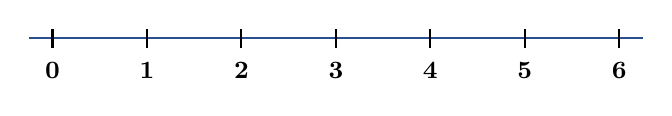
\begin{tikzpicture}
  \draw[thick, scholablue] (0,0) -- (7.8,0);
  \foreach \n in {0,...,6} {
    \draw[thick] (\n*1.2+0.3, -0.12) -- (\n*1.2+0.3, 0.12);
    \node[below] at (\n*1.2+0.3, -0.18) {\small\textbf{\n}};
  }
\end{tikzpicture}

\bigskip

\noindent
\begin{tabular}{@{}p{7.2cm} p{7.2cm}@{}}
% Problem 7: 0+3=3
\textbf{7.}\; Start at 0, hop 3: $0 + 3 =$ \numbox
&
% Problem 8: 1+3=4
\textbf{8.}\; Start at 1, hop 3: $1 + 3 =$ \numbox \\[14pt]

% Problem 9: 2+3=5
\textbf{9.}\; Start at 2, hop 3: $2 + 3 =$ \numbox
&
% Problem 10: 3+3=6
\textbf{10.}\; Start at 3, hop 3: $3 + 3 =$ \numbox \\[14pt]

% Problem 11: 3+2=5
\textbf{11.}\; $3 + 2 =$ \numbox \quad \textit{(use fingers)}
&
% Problem 12: 1+2=3
\textbf{12.}\; $1 + 2 =$ \numbox \quad \textit{(use fingers)}
\end{tabular}

\bigskip\bigskip

% ===== PART III: WRITE YOUR OWN =====
\noindent\textcolor{scholared}{\large\textbf{Part III — Draw and Add}} \hfill \textit{(Problems 13–16)}

\medskip
\noindent\textit{Read the problem. Draw the groups. Write the addition sentence.}

\bigskip

\noindent\textbf{13.} A bird has \textbf{2} eggs. She lays \textbf{2} more. Draw both groups, then write:

\medskip
\noindent\hspace{2em}
\begin{tikzpicture}
  \draw[dashed, scholablue] (0,0) rectangle (4cm, 1.1cm);
  \node[scholablue, right] at (4.2cm, 0.5cm) {\small draw here};
\end{tikzpicture}

\medskip
\noindent\hspace{2em} $\numbox + \numbox = \numbox$

\bigskip

\noindent\textbf{14.} A frog catches \textbf{1} fly, then catches \textbf{3} more. Draw, then write:

\medskip
\noindent\hspace{2em}
\begin{tikzpicture}
  \draw[dashed, scholablue] (0,0) rectangle (4cm, 1.1cm);
\end{tikzpicture}

\medskip
\noindent\hspace{2em} $\numbox + \numbox = \numbox$

\bigskip

\noindent
\begin{tabular}{@{}p{7.2cm} p{7.2cm}@{}}
\textbf{15.} $2 + 3 =$ \numbox & \textbf{16.} $0 + 3 =$ \numbox
\end{tabular}

\bigskip

\begin{enrichbox}
\textbf{\textcolor{scholagreen}{Fact Check — $+0$, $+1$, $+2$, $+3$ to 6}}\\[4pt]
Read aloud with your teacher (no writing — just say the answer!):
\quad $1{+}1$ \quad $2{+}2$ \quad $3{+}3$ \quad $2{+}1$ \quad $3{+}2$ \quad $1{+}3$ \quad $0{+}3$\\[2pt]
\textit{Try to say each answer before your teacher counts to three.}
\end{enrichbox}

\vspace{0.3cm}
\noindent\textcolor{gray}{\small\textit{Ray's Primary Arithmetic — counting on and joining.}}

\end{document}
